\section{The Pixel Cluster Counting (PCC) method}
\label{sec:pcc}

\subsection{Luminosity determination based on PCC}
Pixel cluster counting (PCC)  method is an offline technique for the calculation of instantaneous luminosity $(L_{inst})$ for any LHC run period by counting the number of pixel clusters in the pixel detector (innermost segment of the CMS tracker) in a zero bias event which requires that only two bunches cross at the CMS interaction point. The mean number of pixel clusters $<N_{cl}>$ can be expressed in terms of mean number of pixel clusters per proton-proton interaction  $<N_{cl/pp}>$ and pileup ($\mu$) assuming that clusters do not overlap which is a reasonable assumption given the fine granularity of pixel detector. \\
  
$<N_{cl}> = <N_{cl/pp}> \mu$ \\

$\mu = \frac{<N_{cl}>}{<N_{cl/pp}>}$ \\

The instantaneous luminosity per bunch crossing $L_{b}$ is proportional to the number of proton-proton (pp) interactions per bunch crossing (pileup) and the proportionality constant is the ratio of  LHC orbit frequency f and the pp interaction cross section $\sigma_{pp}$ \cite{CMS-PAS-LUM-12-001}. \\

$L_{b}$ = $\frac{f}{\sigma_{pp}}$ $\mu$  or $L_{b}$ = $\frac{<N_{cl}> \: f }{<N_{cl/pp}> \: \sigma_{pp}}$ \\

The PCC visible cross section $\sigma_{vis}$ which is a calibration constant between pixel clusters rate and luminosity can be defined as \\

$\sigma_{vis}$ = $<N_{cl/pp}>$  $\sigma_{pp}$ \\

Thus, instantaneous luminosity per bunch crossing $L_b$ is given by \\

$L_{b}$ = $\frac{<N_{cl}> \: \sigma_{pp} \: f }{ \:\sigma_{vis} \: \sigma_{pp}}$ or $L_{b}$ = $\frac{<N_{cluster}> \:\: f}{\sigma_{vis}}$ \\

The PCC visible cross section $\sigma_{vis}$ is determined using van der Meer scan method which is described in section 5. Cluster counting can be done over different time periods like per bunch or orbit integrated, 1 Lumi section (23.36s), 4 Lumi nibble (1.46s) and similarly instantaneous luminosity can be calculated over these time periods using PCC method \cite{CMS:2018elu}. \\

\subsection{Run 2018 CMS Data} \\

CMS 2018 data is a collection of runs for each fill in different periods defined during the LHC operation period. LHC 2018 run is divided into A, B, C and D as described below. \\

\begin{flushleft}
1. Run2018A \\
Run number ranges from 315255 to 316995 \\
Number of runs per period is 146 \\
\end{flushleft}

  \begin{flushleft}
2. Run2018B\\
Run number ranges from 317080 to 319311\\
Number of runs per period is 132\\
\end{flushleft}

  \begin{flushleft}
3. Run2018C \\
Run number ranges from 319337 to 320065\\
Number of runs per period is 88 \\
\end{flushleft}

  \begin{flushleft}
4.Run2018D \\
Run number ranges from 320500 to 323699 \\
Number of runs per period is 262 \\
\end{flushleft}

  \begin{flushleft}
5. late Run2018D \\
Run number ranges from 320500 to 325175 \\
Number of runs per period is 339 \\
\end{flushleft}

\subsection{Pixel detector module selection}
Selection of modules in pixel detector is required because module may experience dynamic inefficiency, bad module chips can stop sending data, chips may not work properly and need reconfiguring. Modules which are observed to function efficiently are considered for luminosity estimation. The module veto lists correspond to late Run2018D that select each detector part barrel layers L2, L3, L4 and forward disks D1, D2, D3 as shown in Fig. 12 and 13. Barrel layer 1 (L1) is not used for luminosity determination \cite{vetolist}. \\

\begin{flushleft}
Total number of modules: 1856 \\
BPIX modules per layer:  96 , 224 , 352 , 512\\
FPIX modules per disk:  112 , 112 , 112 , 112 , 112 , 112\\
\end{flushleft}

\begin{figure}[H]
  \centering
  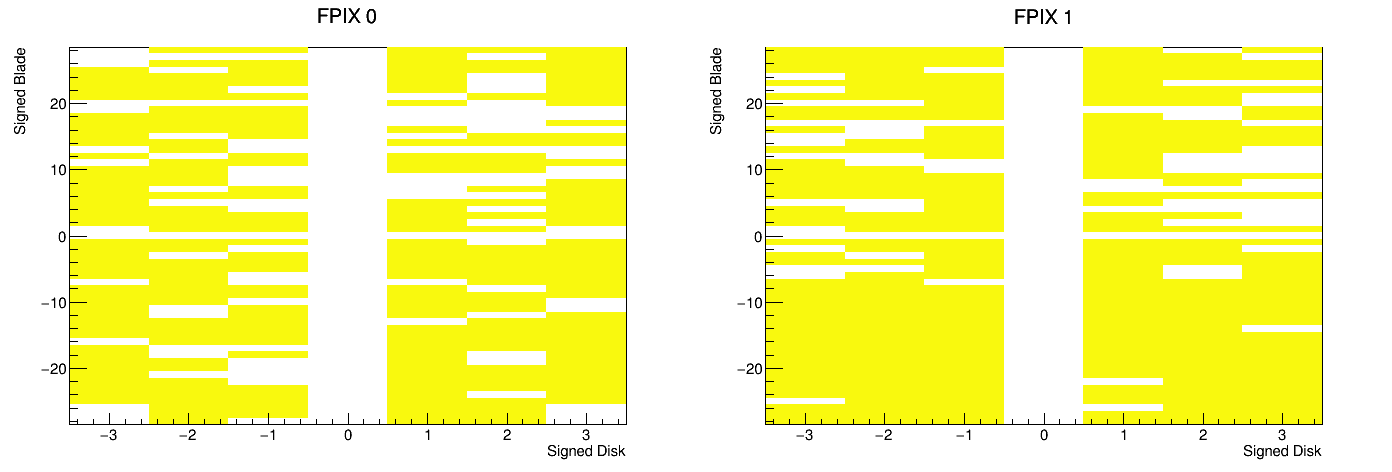
\includegraphics[width=0.8 \columnwidth]{./PDDisk_R12.png}
  \caption{ \onehalfspacing Diagram showing coordinates of modules in one forward disk of pixel detector having two rings. FPIX 0 correspond to ring 1 and FPIX 1 to ring 2. Yellow regions shows coordinates of vetoed modules while white regions shows coordinates of good modules used for luminosity determination.}
  \label{fig:CMS}
\end{figure}

\begin{figure}[H]
  \centering
  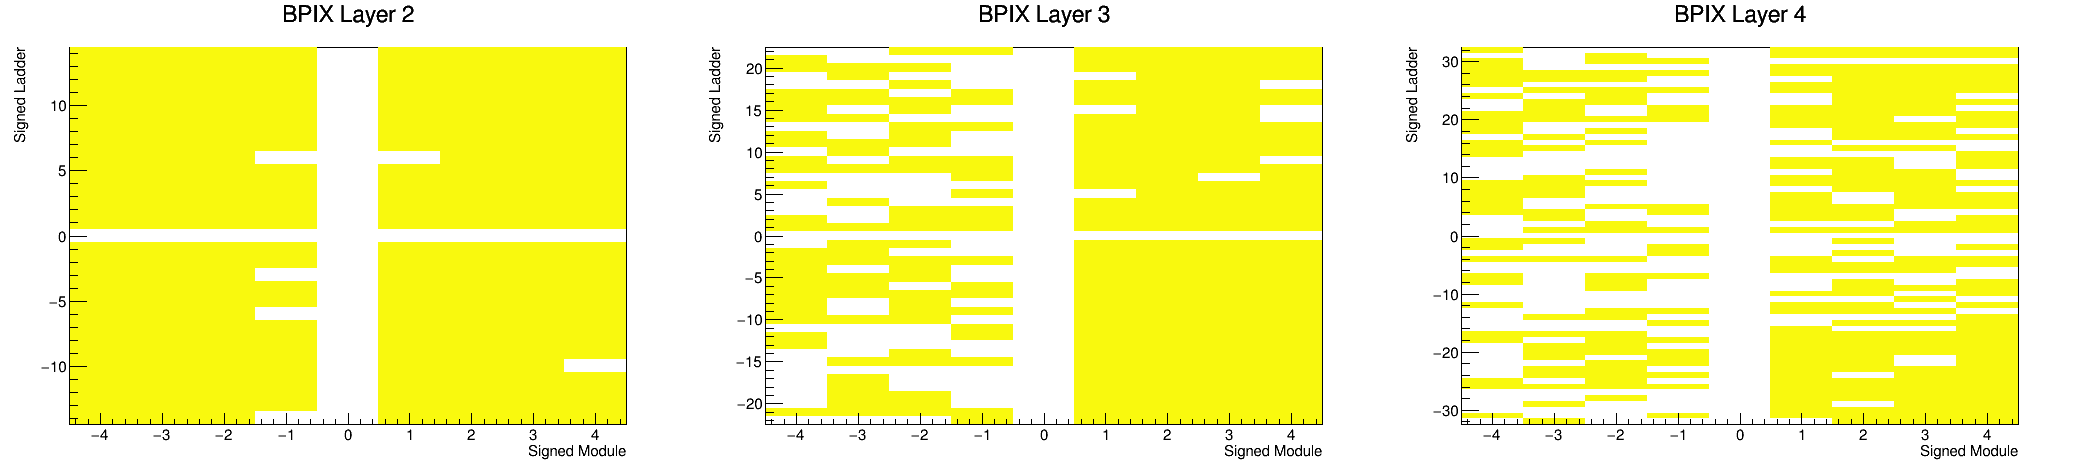
\includegraphics[width=1 \columnwidth]{./bpixL2-L4.png}
  \caption{ \onehalfspacing Diagram showing z coordinate (signed module) and phi coordinate (signed ladder) of modules in three barrel layers (L2, L3 and L4) of pixel detector. Yellow regions shows coordinates of vetoed modules while white regions shows coordinates of good modules used in luminosity determination. }
  \label{fig:CMS}
\end{figure}




\clearpage\newpage

